\chapter{Classical Problems}
\section{Review of Basic Concept}
\begin{enumerate}
	\item At the moment $t=0$ a stationary particle of mass $m$ experiences a time-dependent force $F=k t\left(t^{\prime}-t\right)$, where $k$ is a constant vector, $t^{\prime}$ is the time during which the given force acts. Find :\\
	(a) the momentum of the particle when the action of the force discontinued;\\
	(b) the distance covered by particle while the force acted.
	\begin{answer}
	(a) Since $F=k t\left(t^{\prime}-t\right)$, the direction of the force is fixed, as $k$ is a constant vector and the particle starts from rest, the motion will be in the direction of the force.
	\begin{align*}
	m \frac{d v}{d t}&=k t\left(t^{\prime}-t\right),\text{ from Newton's II law}\\
	\text{Integrating, }\int_{0}^{v} d v&=\frac{k}{m} \int_{0}^{t^{\prime}} t\left(t^{\prime}-t\right) d t=\frac{k}{m}\left[t^{\prime} \frac{t^{2}}{2}-\frac{t^{3}}{3}\right]_{0}^{t^{\prime}} \quad v=\frac{k}{m} \cdot \frac{t^{\prime 3}}{6}\\
\text{	Therefore, momentum of the particle }p&=m v=k t \frac{t^{\prime 3}}{6}.\\
\text{(b) }d s=v d t \Rightarrow s&=\int_{0}^{s} d s=\int_{0}^{t^{\prime}} v d t=\frac{k t^{\prime 4}}{12 m}
	\end{align*}
		\end{answer}
	\item A block of mass $m_{1}=4 \mathrm{~kg}$ on a smooth inclined plane of $30^{\circ}$ is connected by a cord over a small, frictionless pulley to a second block of mass $m_{2}=5 \mathrm{~kg}$ hanging vertically. Calculate the acceleration with which the block moves and also the tension in the cord. Take $g=10 \mathrm{~m} / \mathrm{sec}^{2}$.
	\begin{answer}
			The different forces acting on the masses are shown in figure.
			\begin{figure}[H]
				\centering
				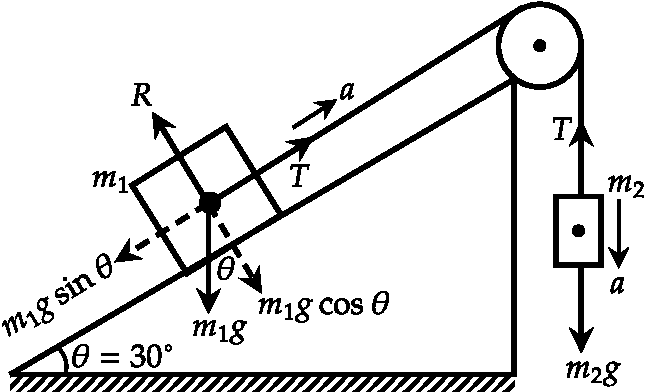
\includegraphics[height=3.5cm,width=6cm]{diagram-20220216-crop}
			\end{figure}
		\begin{align}
\text{We have }T-m_{1} g \sin \theta&=m_{1} a \label{1} \\
\text{ and }m_{2} g-T&=m_{2} a \label{2}\\
\intertext{Solving equations (\ref{1}) and (\ref{2}), we get}
a&=\frac{\left(m_{2}-m_{1} \sin \theta\right) g}{\left(m_{1}+m_{2}\right)}\label{3}\\
\text { and } \quad T & =m_{2} g\left[1-\frac{\left(m_{2}-m_{1} \sin \theta\right)}{\left(m_{1}+m_{2}\right)}\right] \notag\\
 \text { or } \quad T & =\frac{m_{1} m_{2}(1+\sin \theta) g}{\left(m_{1}+m_{2}\right)}\\
 \text{Here }m_{1}&=4 \mathrm{~kg}, m_{2}=5 \mathrm{~kg}, \theta=30^{\circ} \text{and }g=10 \mathrm{~m} / \mathrm{s}\notag\\
  \intertext{Substituting these values in equation (\ref{3}), we get}
 T&=\frac{5 \times 4\left(1+\frac{1}{2}\right) 10}{9}=\frac{300}{9}=33.33 \mathrm{~N}\notag
\end{align}
	\end{answer}
	\item A particle of mass $m$ is connected to two springs of unstretched length ' $l$ ' and spring constant $k$ as show in figure. Calculate acceleration of particle if it is slightly displaced along X-direction.
	\begin{answer}
			Let the particle is displaced by a distance $x$ along $+x$ direction as shown in figure.
			\begin{figure}[H]
				\centering
				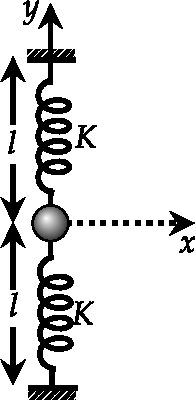
\includegraphics[height=4.5cm,width=2cm]{diagram-20220216(1)-crop}
			\end{figure}
		\begin{figure}[H]
			\centering
			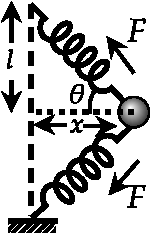
\includegraphics[height=3cm,width=2cm]{diagram-20220216(2)-crop}
		\end{figure}
		\begin{align*}
	\text{	Therefore, stretched length of spring }&=\sqrt{l^{2}+x^{2}}\\
		\text{elongation in springs }&=\sqrt{l^{2}+x^{2}}-l\\
	\text{	Restoring force on the particle due to each spring} F&=k\left(\sqrt{l^{2}+x^{2}}-l\right)
	\intertext{ Because of restoring force the particle moves back towards its initial position.}
\text{	Equation of motion of particle }F_{x}&=m \frac{d^{2} x}{d t^{2}}\\
	\text{or }-2 F \cos \theta&=m \frac{d^{2} x}{d t^{2}}\text{ or }-2 k\left(\sqrt{l^{2}+x^{2}}-l\right) \cdot \frac{x}{\sqrt{l^{2}+x^{2}}}=m \frac{d^{2} x}{d t^{2}}\\
	\text{Therefore, }\frac{d^{2} x}{d t^{2}}&=-\frac{2 k x}{m}\left(1-\frac{l}{\sqrt{l^{2}+x^{2}}}\right)\text{ or }\frac{d^{2} x}{d t^{2}}\\&=-\frac{2 k x}{m}\left[1-\left(1+\frac{x^{2}}{l^{2}}\right)^{-1 / 2}\right]\\
\text{	Since, }&x<l,\left(1+\frac{x^{2}}{l^{2}}\right)^{-1 / 2} \approx 1-\frac{x^{2}}{2 l^{2}}\\
\text{	Therefore, }\frac{d^{2} x}{d t^{2}}&=-\frac{2 k x}{m}\left[1-\left(1-\frac{x^{2}}{2 l^{2}}\right)\right]\text{ or }\frac{d^{2} x}{d t^{2}}=-\frac{k x^{3}}{m l^{2}}
		\end{align*}
	\end{answer}
\item At the moment $t=0$, the force $F=k t$ is applied to a small body of mass $m$ resting on smooth horizontal plane $(k=$ constant). The permanent direction of this force forms an angle $\theta$ with the horizontal (figure below). Find\\
\begin{figure}[H]
	\centering
	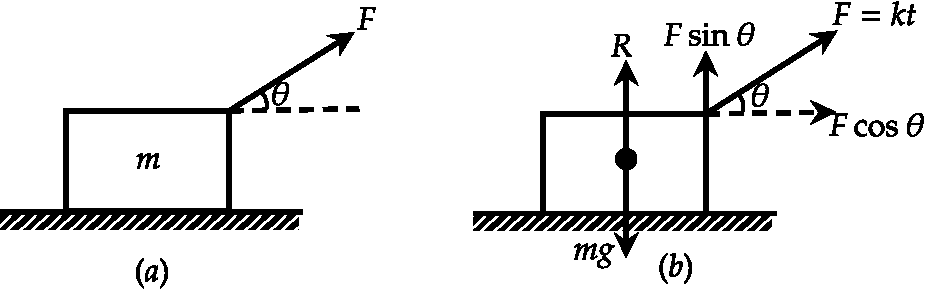
\includegraphics[height=3cm,width=10cm]{diagram-20220217-crop}
\end{figure}
(a) the velocity of the body at the moment of its breaking off the plane;\\
(b) the distance traversed by the body up to this moment.

\begin{answer}
		The free body diagram is shown in figure.
	\begin{align*}
	\text{From figure: }R+F \sin \theta&=m g\\
	\text{At breaking off, }R&=0, \therefore F=\frac{m g}{\sin \theta}\\
\text{	Now }k t&=\frac{m g}{\sin \theta}\text{ or }t=\frac{m g}{k \sin \theta}
\intertext{	(a) If $a$ be the acceleration, then $F \cos \theta=m a$ }
\text{	Therefore, }k t \cos \theta&=m \times\left(\frac{d v}{d t}\right) \quad\left(\because a=\frac{d v}{d t}\right) .
\intertext{Integrating this expression within proper limits, we get $m \int_{0}^{v} d v=k \cos \theta \int_{0}^{m g / k \sin \theta} t d t$}
\text{ or }\quad m v&=\frac{k \cos \theta}{2}\left[\frac{m g}{k \sin \theta}\right]^{2}\text{ or }v=\frac{m g^{2}}{2 k}\left(\frac{\cos \theta}{\sin ^{2} \theta}\right)\\
\text{(b) Without putting the limits, we have }v&=\frac{k \cos \theta}{2 m} t^{2}+C,\text{ where $C=$ constant of integration.}\\
\text{When }t&=0, v=0\text{ and hence }C=0.\\
\text{Now, }\frac{d s}{d t}&=\frac{k \cos \theta}{2 m} t^{2} \int_{0}^{s} d s=\frac{k \cos \theta}{2 m} \int_{0}^{m g / k \sin \theta} t^{2} d t\\
s&=\frac{k \cos \theta}{2 m}\left[\frac{t^{3}}{3}\right]_{0}^{m g / k \sin \theta} \quad\text{ or }s=\frac{m^{2} g^{3} \cos \theta}{6 k^{2} \sin ^{3} \theta} .
	\end{align*}
\end{answer}
\item Spherical particles of a given material of density $\rho$ are released from rest inside a liquid medium of lower density. The viscous drag force may be approximated by the Stoke's law, i.e, $F_{d}=6 \pi \eta R \mathrm{v}$, where $\eta$ is the viscosity of the medium, $R$ the radius of a particle and $v$ its instantaneous velocity. If $\tau(m)$ is the time taken by a particle of mass $m$ to reach half its terminal velocity, then the ratio $\tau(8 m) / \tau(m)$ is
\begin{answer}
	 Each particle has same density but different radii and masses. We have to calculate time of fall in terms of mass of particle therefore we will write our equations explicitly in terms of mass and we will remove radius from our equations wherever it appears.\\Drag force on particles
	 \begin{align}
	 F_{d}&=6 \pi \eta R \mathrm{v}, \quad\text{ Mass of a particle }m=\rho \cdot \frac{4}{3} \pi R^{3}\notag\\
	 \therefore R&=\left(\frac{3 m}{4 \pi \rho}\right)^{1 / 3} \quad \therefore F_{d}\notag\\&=6 \pi \eta\left(\frac{3 m}{4 \pi \rho}\right)^{1 / 3} v=K m^{1 / 3} v\text{, where }K=6 \pi \eta\left(\frac{3}{4 \pi \rho}\right)^{1 / 3}\notag\\
	\intertext{ If $\mathrm{B}$ is buoyancy force, then equation of motion of a particle is}\notag\\
	 m \frac{d v}{d t}&=m g-F_{d}-B\text{ where }\mathrm{B}=\frac{4}{3} \pi R^{3} \sigma g\notag\\&=\frac{4}{3} \pi R^{3} \rho g \cdot \frac{\sigma}{\rho}=m g \frac{\sigma}{\rho}, \sigma=\text{ density of medium}\notag\\
	 \therefore m \frac{d v}{d t}&=m g-K m^{1 / 3} v-m g \frac{\sigma}{\rho}, m \frac{d v}{d t}=m g\left(1-\frac{\sigma}{\rho}\right)-K m^{1 / 3} v \notag\\
	 \text { or } \frac{d v}{d t}&=g\left(1-\frac{\sigma}{\rho}\right)-K m^{-2 / 3} v\label{5}\\
	 \text{when terminal }&\text{velocity is reached }\frac{d v}{d t}=0\notag\\
	 \therefore 0&=g\left(1-\frac{\sigma}{\rho}\right)-K m^{-2 / 3} v_{t} \quad \therefore v_{t}=\frac{g\left(1-\frac{\sigma}{\rho}\right)}{K m^{-2 / 3}}\label{6}\\
	\intertext{ Now, if $\tau$ be the time to reach half the terminal velocity then from (\ref{5})}\notag\\
	 \int_{0}^{1 / 2} \frac{d v}{g\left(1-\frac{\sigma}{\rho}\right)-K m^{-2 / 3} v}&=\int_{0}^{\tau} d t, \quad \therefore-\frac{1}{K m^{-2 / 3}} \ln \left[\frac{g\left(1-\frac{\sigma}{\rho}\right)-\frac{K m^{-2 / 3} v_{t}}{2}}{g\left(1-\frac{\sigma}{\rho}\right)}\right]=\tau\notag\\
	 \text{using value of $v_{t}$ from (\ref{6}) we get, }\tau&=\frac{m^{2 / 3}}{K} \ln 2 \quad\text{ or }\quad \tau(m)=\frac{m^{2 / 3} \ln 2}{K}\notag\\
	  \therefore \tau(8 m) / \tau(m)&=(8 m)^{2 / 3} / m^{2 / 3}=4\notag
	 \end{align}
\end{answer}
\item A particle of unit mass is thrown vertically upward with initial speed $v_{0}$. It is acted upon by a drag force $b v^{2}$ in addition to gravity where $b$ is constant and $v$ is instantaneous velocity of particle. Calculate speed of the particle when it returns to the point from where it was thrown.
\begin{answer}
	In presence of drag force only quantity that is common in upward and downward motion is the distance covered.
	\begin{figure}[H]
		\centering
		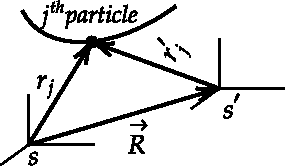
\includegraphics[height=3cm,width=7cm]{diagram-20220218-crop}
	\end{figure}
	\begin{align*}
	\text{For upward motion, initial speed }&=v_{0},\\
	 \text{final speed }&=0,\text{ let height reached $=h$}\\
	 \text{ equation of motion }\frac{d v}{d t}&=-g-b v^{2}\\
	\text{or }\frac{d v}{d y} \cdot \frac{d y}{d t}&=-g-b v^{3}, \frac{d y}{d t}=v\text{ or }\frac{v d v}{g+b v^{2}}=-d y\\
	\therefore \int_{v}^{0} \frac{v d v}{g+b v^{2}}&=-\int_{0}^{h} d y\\
\text{	on integration we get, }\frac{1}{2 b} \ln \left(\frac{g+b v_{0}^{2}}{g}\right)&=h\\
\text{for downward motion, initial speed }&=0,\text{ final speed $=v($ let $)$, height descended $=h$ }\\
\text{equation of motion }\frac{d v}{d t}&=g-b v^{2}\text{ or }\frac{v d v}{g-b v^{2}}=d y\text{ or }\int_{0}^{v} \frac{v d v}{g-b v^{2}}=\int_{0}^{h} d y\\
\text{on integration we get, }\frac{1}{2 b} \ln \left(\frac{g}{g-b v^{2}}\right)&=h\\
\text{Comparing (a) and (b) we get, }\frac{g+b v_{0}^{2}}{g}&=\frac{g}{g-b v^{2}}, \quad g-b v^{2}=\frac{g^{2}}{g+b v_{0}^{2}}\\
\text{or }v&=\frac{v_{0}}{\sqrt{1+\frac{b v_{0}^{2}}{g}}} \Rightarrow v<v_{0}
	\end{align*}
	due to drag force the particle returns with a speed less than its initial speed. If drag force were absent $b=0$, then $v=v_{0} .$ Therefore in absence of drag force particle returns with same speed as its initial value.
\end{answer}
\item A small ring of mass $m$ can slide on a smooth circular wire of radius $r$ and center $O$, which is fixed in a vertical plane. From a point on the wire at a vertical distance $r / 2$ above $O$, the ring is given a velocity $\sqrt{(g r) }\text { along the downward tangent to the wire. Show that it will just reach the highest point of the wire. }$ Find the reaction between the ring and the wire when the ring is at a vertical distance $r / 2$ below.
\begin{answer}
	\begin{align}
\text{At point $C$, the velocity of the ring }&=\sqrt{(r g)}.\notag\\
\text{K.E. at }C&=\frac{1}{2} m v^{2}=\frac{1}{2} m r g\text{ and P.E. at }C\notag\\&=m g h=m g(A F)=m g(r+r / 2)=\frac{3 m g r}{2}.\notag\\
\text{Total energy }&=m g r\left[\frac{1}{2}+\frac{3}{2}\right]=2 m g r.\label{7}
	\end{align}
	If the ring has to reach at $D$, with kinetic energy zero, its potential energy $=m g(2 r)$.
	Becuase the particle at $C$ has this amount of energy and it will just reach at $D$ with zero velocity.\\
	\begin{figure}[H]
		\centering
		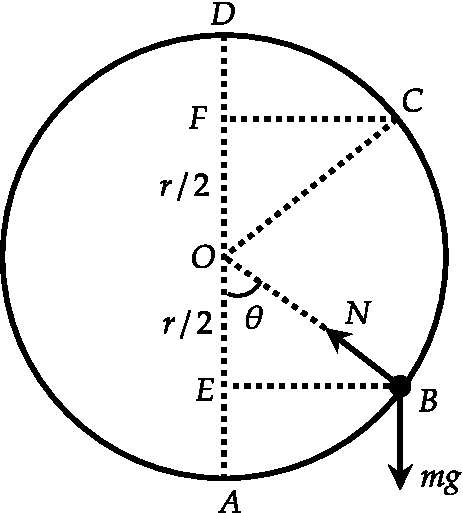
\includegraphics[height=4.8cm,width=4.5cm]{diagram-20220217(1)-crop}
	\end{figure}
	Now consider the ring at $B$, a distance $r / 2$ below $O$. Resolving $m g$ in two parts and considering the equilibrium, we get
	\begin{align}
	N-m g \cos \theta&=\frac{m v_{1}^{2}}{r}\notag\\
	N&=\frac{m v_{1}^{2}}{r}+m g \cos \theta\label{8}
	\intertext{Falling from $C$, i.e., through a distance $r$, the ring has lost a potential energy $m g r .$ This is the gain in kinetic energy.}
\text{	Hence, }\frac{1}{2} m v_{1}^{2}&=\frac{1}{2} m g r+m g r=\frac{3}{2} m g r \text{or }v_{1}^{2}=3 g r\text{ or }\frac{v_{1}^{2}}{r}=3 g.\notag\\
\text{ Fromequation (\ref{8}),} N&=m\left(3 g+g \times \frac{1}{2}\right)
	\left(\because \cos \theta=\frac{1}{2}\right)\notag\\\text{ or}& N=\left(\frac{7}{2}\right) \mathrm{mg}=3.5 \mathrm{mg}.\notag
	\end{align}
\end{answer}
\item A $2.0 \mathrm{~kg}$ block of mass, initially at rest, is dropped from a height of $0.40$ meter onto a spring whose force constant is $1960 \mathrm{nt} /$ meter. Find the maximum distance that the spring will be compressed.
\begin{answer}
	The situation is shown in figure. Let $m$ be the mass of the block and $k$ be the force constant of the spring.Let $l$ be the distance through which the spring is compressed. The total vertical fall of the block is $(h+l)$. Loss of the gravitational potential energy of the block $=m g(h+l)$.\\
	\begin{figure}[H]
		\centering
		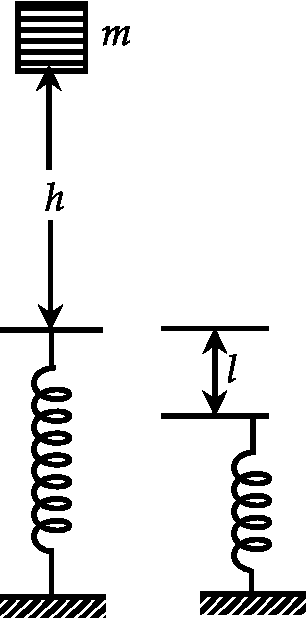
\includegraphics[height=5cm,width=2.5cm]{diagram-20220217(2)-crop}
	\end{figure}
	\begin{align*}
	\text{Elastic potential energy }&\text{in the spring }=\left(\frac{1}{2}\right) k t^{2}.
\intertext{	By the law of conservation of energy}
	m g(h+l)&=\frac{1}{2} k t^{2} \text { or } \frac{2 m g h}{k}+\frac{2 m g}{k} l=l^{2} \text { or } l^{2}-\frac{2 m g}{k} l-\frac{2 m g h}{k}=0\\
	\therefore \quad l&=\frac{\left(\frac{2 m g}{k}\right) \pm \sqrt{\left[\left(\frac{2 m g}{k}\right)^{2}+\left(\frac{8 m g h}{k}\right)\right]}}{2}\\
	\text{According to given problem, }m&=2 \mathrm{~kg}, h=0.40 \mathrm{~m} \text{and $k=1960$ newton/meter. Hence,}\\
	l&=\frac{(2 \times 2 \times 9.8 / 1960) \pm \sqrt{(2 \times 2 \times 9.8 / 1960)^{2}+(8 \times 2 \times 9.8 \times 0.40 / 1960)}}{2} \\
	l&=\mathbf{0 . 1} \text { meter. }
	\end{align*}
\end{answer}
\item A particle of mass $3 \mathrm{~kg}$ is moving under the action of a central force whose potential energy is given by $U(r)=10 r^{3}$ joule. For what energy and angular momentum will the orbit be a circle of radius $10 \mathrm{~m}$ ? Calculate the time period of this motion.
\begin{answer}
	\begin{align*}
	\text{Given that }U(r)&=10 r^{3}.
	\intertext{So the force $F$ acting on the particle is given by}
	F&=\frac{\partial U}{\partial r}=-\frac{\partial}{\partial r}\left(10 r^{3}\right)=-10 \times 3 r^{2}=-30 r^{2}\\
	\text{For circular motion of the particle }F&=\frac{m v^{2}}{r}=30 r^{2}.\\
	\text{Substituting the given values, we have }\frac{3 \times v^{2}}{10}&=30 \times(10)^{2}\text{ or }v=100 \mathrm{~m} / \mathrm{s}.\\
	\text{The total energy in circular motion}
	E&=\text{ K.E. }+\text{ P.E. }=\frac{1}{2} m v^{2}+U(r)\\&=\frac{1}{2} \times 3 \times(100)^{2}+10 \times(10)^{3}=2.5 \times 10^{4}\text{ joule}\\
	\text{Angular momentum }&=m v r=3 \times 100 \times 10=3000 \mathrm{~kg}-\mathrm{m}^{2} / \mathrm{sec}\\
	\text{Time period }T&=\frac{2 \pi r}{v}=\frac{2 \times \pi \times 10}{100}=\frac{\pi}{5} \mathrm{sec} .
	\end{align*}
\end{answer}
\item In figure, $A B C D E$ is a channel in the vertical plane, part $B C D E$ being circular with radius $r$. A ball is released from $A$ and slides without friction and without rolling. Show that it will complete the loop path if $h$ is greater than $5 r / 2$.
\begin{figure}[H]
	\centering
	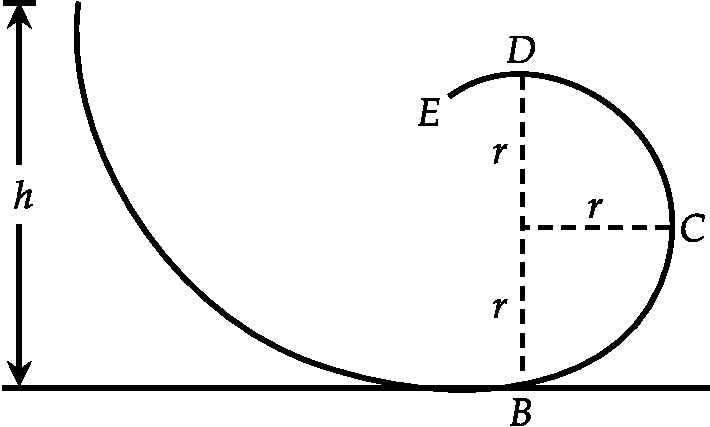
\includegraphics[height=3cm,width=5cm]{diagram-20220217(3)-crop}
\end{figure}
\begin{answer}
	\begin{align}
\intertext{	Let $m$ be the mass of the ball. When the ball comes down to $B$, its loses its potential energy $m g h$ which is converted into kinetic energy. Let $v_{B}$, be the velocity of the ball at $B$. Then,}\notag\\
	m g h&=\frac{1}{2} m v_{B}^{2}
\intertext{	The ball now rises to a point $D$, where its potential energy is $m g(h-2 r) .$ If $v_{D}$ be the velocity of the ball at $D$, then}\notag\\
	m g(h-2 r)&=\frac{1}{2} m v_{D}^{2}\label{09}
\intertext{	Now to complete the circular path, it is necessary that the centripetal force acting upward at point $D$ should be equal or greater than the force $m g$ acting downward. Therefore,}\notag\\
	\frac{m v_{D}^{2}}{r} \geq m g&\text{ or }v_{D}^{2} \geq r g\\
\text{	Fromequation (\ref{09}) }v_{D}^{2}&=2 g(h-2 r)\notag\\
	\therefore \quad 2 g(h-2 r) \geq &r g, h \geq \frac{5}{2} r .\notag
	\end{align}
\end{answer}
\item A moving particle of mass $m$ collides head-on with a particle of mass $2 m$ which is initially at rest. Show that the particle $m$ will loose $8 / 9$ th part of its initial kinetic energy after the collision.
\begin{answer}
	Let $u_{1}$ be the initial velocity of mass $m$ before collision and $v_{1}$ and $v_{2}$ the velocities of masses $m$ and $2 m$ after collision respectively.\\
	According to the law of conservation of kinetic energy, we have
	\begin{align}
 \frac{1}{2} m u_{1}^{2}&=\frac{1}{2} m v_{1}^{2}+\frac{1}{2}(2 m) v_{2}^{2}\notag \\ \text { or } & u_{1}^{2}-v_{1}^{2}=2 v_{2}^{2} \notag\\ \text { or } & \left(u_{1}-v_{1}\right)\left(u_{1}+v_{1}\right)=2 v_{2}^{2}\label{10}
\intertext{ By the law of conservation of momentum, we have}\notag
 m u_{1}&=m v_{1}+(2 m) v_{2} \notag\\
 \left(u_{1}-v_{1}\right)&=2 v_{2}\label{11}\\
\text{ From eqs. (\ref{10}) and (\ref{11}), we get }\left(u_{1}+v_{1}\right)&=v_{2}\label{12}
\intertext{ Substituting the value of $v_{2}$ from eq. (\ref{12}) in eq. (\ref{11}), we get}\notag\\
u_{1}-v_{1}=2\left(u_{1}+v_{1}\right) \text { or }-3 v_{1}&=u_{1} \text { or } v_{1}=-\left(\frac{1}{3}\right) u_{1}\label{13}
\intertext{Now the initial and final kinetic energies of mass $m$ are}
K_{i}=\left(\frac{1}{2}\right) m u_{1}^{2} \text { and } K_{f}&=\left(\frac{1}{2}\right) m v_{1}^{2}=\left(\frac{1}{2}\right) m\left(\frac{u_{1}^{2}}{9}\right)\notag\\
\text{Therefore, fraction loss }&=\frac{K_{i}-K_{f}}{K_{i}}=\frac{\frac{1}{2} m u_{1}^{2}\left(1-\frac{1}{9}\right)}{\frac{1}{2} m u_{1}^{2}}=\frac{8}{9}\notag
	\end{align}
\end{answer}
\item A solid hemisphere of mass $M$ and radius $R$ is placed against a smooth wall as shown in the figure. what is normal reaction on the sphere due to the wall.
\begin{answer}
	Centre of mass of the hemisphere lies at a distance $\frac{3 R}{8}$ from
	its base centre. The sphere is in equilibrium therefore torque about point A must be zero.
	\begin{figure}[H]
		\centering
		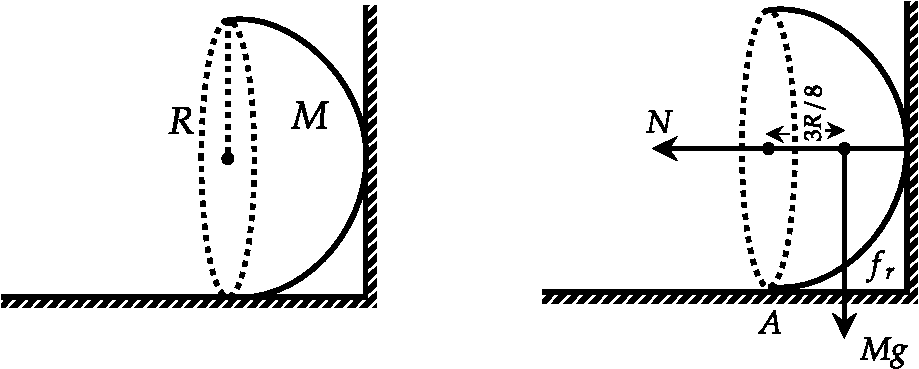
\includegraphics[height=3.2cm,width=9cm]{diagram-20220217(4)-crop}
	\end{figure}
	\begin{align*}
	\therefore N R-M g \cdot \frac{3 R}{8}&=0\\
	\text{or, }N&=\frac{3 M g}{8}
	\end{align*}
\end{answer}
\item A thin rod of mass $M$ and length $L$ is suspended from one end while its other end lies on a smooth horizontal plane and makes an angle $\alpha$ with the plane. Find the normal reaction from the plane and tension in the string from which it is suspended.
\begin{figure}[H]
	\centering
	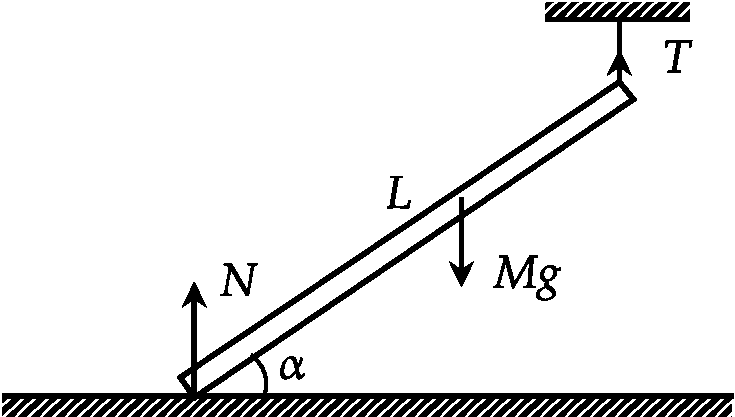
\includegraphics[height=3cm,width=5cm]{diagram-20220217(5)-crop}
\end{figure}
\begin{align}
\text{For translational equilibrium }T+N&=M g \label{14}\\
\text{For rotational }&\text{equilibrium }\notag\\
\text{Torque about lower}&\text{ end of the rod is zero}\notag\\
	\therefore T . L \cos \alpha-M g \frac{L}{2} \cos \alpha&=0 \quad \therefore \quad T=\frac{M g}{2}\notag\\
	\text{from (\ref{14}) }N&=M g-T=M g-\frac{M g}{2}=\frac{M g}{2}\notag
\end{align}
Example: A uniform ladder of length 2L and mass 'm' leans against a wall in a vertical plane at an angle $\theta$ to the horizontal. The floor is rough, having a coefficient of static friction $\mu$
A person of mass $M$ stands on the ladder at a distance $D$ from its base (see figure). If the wall is frictionless, the maximum distance $\left(D_{\max }\right)$ up the ladder that the person can reach before the ladder slips is
\begin{figure}[H]
	\centering
	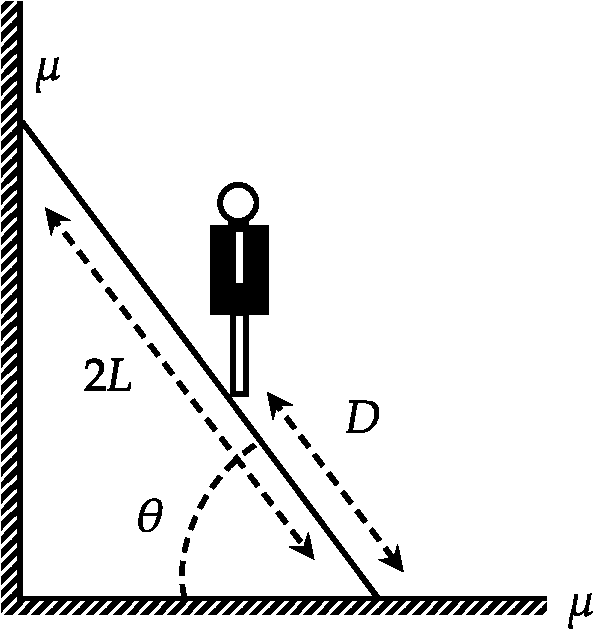
\includegraphics[height=4cm,width=4cm]{diagram-20220217(6)-crop}
\end{figure}
\begin{answer}
	Let us take ladder plus person as system. Various forces acting on the system are shown in the figure. For translational equilibrium we must have
	\begin{align}
	N_{1}&=(M+m) g\label{15}\\
	N_{2}&=f_{r}\label{16}\\
	\intertext{	For rotational equilibrium torque about lower end of the ladder must be zero. Therefore,}\notag\\
	M g D \cos \theta+m g L \cos \theta-N_{2} .2 L \sin \theta&=0\notag\\
	\therefore N_{2}&=\frac{g \cot \theta}{2}\left[\frac{M D}{L}+m\right]\notag\\
	\therefore\text{ from (\ref{16}) we get, }f_{r}&=\frac{g \cot \theta}{2}\left[\frac{D}{L} M+m\right]\notag\\
	\text{since }f_{r} \leq \mu N_{1}, \quad &\therefore \frac{g \cot \theta}{2}\left[\frac{D}{L} M+m\right] \leq \mu(M+m) g\notag\\
\text{	or }D \leq \frac{L}{M}[2 \mu(M+m) \tan \theta-m] \quad &\therefore D_{\max }=L\left[2 \mu\left(1+\frac{m}{M}\right) \tan \theta-\frac{m}{M}\right]\notag
	\end{align}
 \begin{figure}[H]
 	\centering
 	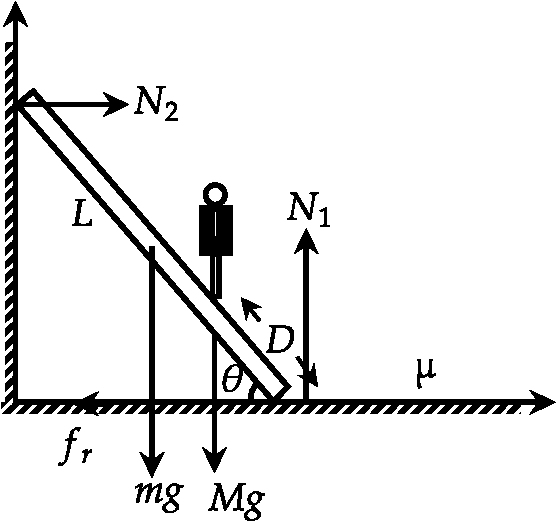
\includegraphics[height=4.5cm,width=4.5cm]{diagram-20220217(7)-crop}
 \end{figure}
\end{answer}
\item A body of mass $m$ rests on a horizontal plane with the friction coefficient $\mu .$ At the moment $t=0$, a horizontal force is applied to it, which varies with time $F=k t$, where $k$ is a constant vector. Find the distance traversed by the body during first/seconds after the force action began.
\begin{answer}
	Here just after applying the force, the motion does not start due to friction force. As the applied force is proportional to time, let after a time $t_{0}$, the motion starts.
	\begin{align*}
	\text{Now, }F=k t_{0}=\mu m g\text{ or }t_{0}=\left(\frac{\mu m g}{k}\right)
\intertext{	If $t \leq t_{0}$, the distance traversed by the body $s=0 .$}
\text{	When }t \leq t_{0},\text{ then }F&=k\left(t-t_{0}\right)
	\end{align*}
		\begin{align}
	\therefore \quad m \frac{d v}{d t}&=k\left(t-t_{0}\right)\text{ or }m d v=k\left(t-t_{0}\right) d t \ldots \label{17}\\
\text{	Integrating equation (\ref{17}), we get } m v&=\frac{k}{2}\left(t-t_{0}\right)^{2}+C_{1}\notag\\
	\text{When }t&=t_{0}, v=0, \therefore C_{1}=0\notag\\
	\therefore \quad m v&=\frac{k}{2}\left(t-t_{0}\right)^{2}\\
	\text{Again }m \frac{d s}{d t}&=\frac{k}{2}\left(t-t_{0}\right)^{2}\text{ or }m d s=\frac{k}{2}\left(t-t_{0}\right)^{2} d t\label{19}\\
	\text{Integrating equation (\ref{19}), we get }s&=\frac{k}{6 m}\left(t-t_{0}\right)^{3}+C_{2}\notag\\
\text{	Here }C_{2}&=0\text{ because when }t=t_{0}, s=0\notag\\
	\therefore \quad s&=\frac{k}{6 m}\left(t-t_{0}\right)^{3} .\notag
	\end{align}
\end{answer}
\item A falling rain drop accumulates moisture due to which its radius increases at a constant rate $k$. Neglecting drag calculate the speed of rain drop after it has fallen for a time $t$.
\begin{answer}
	\begin{align}
	\text{Equation of motion }\frac{d p}{d t}&=m g\label{20}\\
	\text{given }\frac{d r}{d t}&=k \Rightarrow r=k t\text{ (if initial radius is zero)}\notag\\
	\text{since }m&=\frac{4}{3} \pi r^{3} \rho \quad \therefore \frac{d m}{d t}=4 \pi r^{2} \cdot \frac{d r}{d t} \cdot \rho\notag
\intertext{	$\rho$ is density, we assume it to be constant}\notag
	\frac{d m}{d t} &=\left(\frac{4}{3} \pi r^{3} \rho\right) \cdot \frac{3 k}{r} \notag\\
	\frac{d m}{d t} &=\frac{3 m k}{r}\label{21}\\
\intertext{	Dividing (\ref{20}) by (\ref{21}) we get}\notag
\frac{d p}{d m}&=\frac{g}{3 k} r \quad d p=\left(\frac{g}{3 k}\right) \cdot\left(\frac{3 m}{4 \pi \rho}\right)^{1 / 3} d m\notag\\
\intertext{on integration we get}\notag
\therefore \quad p&=\left(\frac{g}{3 k}\right)\left(\frac{3}{4 \pi \rho}\right)^{1 / 3} \cdot \frac{m^{4 / 3}}{4 / 3}+c\notag\\
\text{taking }p&=m=0\text{ at }t=0,\text{ we get }c=0\notag\\
\therefore \quad p&=\frac{g}{4 k}\left(\frac{3}{4 \pi \rho}\right)^{1 / 3} \cdot m^{4 / 3}\notag\\
\text{or }v&=\left(\frac{g}{4 k}\right) \cdot\left(\frac{3 m}{4 \pi \rho}\right)^{1 / 3}\notag\\
v&=\frac{g}{4 k} r \Rightarrow v=\frac{g}{4} t\notag
	\end{align}
\end{answer}
	\item A particle of mass $2 \mathrm{~kg}$ is moving such that at time $t$, its position, in metre, is given by $\vec{r}(t)=5 \hat{i}-2 t^{2} \hat{j}$. The angular momentum of the particle at $t=2 \mathrm{~s}$ about the origin, in $\mathrm{kg} \mathrm{m}^{2} \mathrm{~s}^{-1}$, is
	 \begin{tasks}(2)
		\task[\textbf{a.}]$-40 \hat{k}$
		\task[\textbf{b.}]$-80 \hat{k}$
		\task[\textbf{c.}]$80 \hat{k}$
		\task[\textbf{d.}]  $40 \hat{k}$
	\end{tasks}
	\begin{answer}
		\begin{align*}
		\vec{r} &=5 \hat{i}-2 t^{2} \hat{j} \\
		\vec{v} &=\frac{d \vec{r}}{d t}=-4 t \hat{j} \\
		\vec{p} &=m \vec{v}=2(-4 t \hat{j})=-8 t \hat{j} \\
		\vec{L} &=\vec{r} \times \vec{p}=\left(5 \hat{i}-2 t^{2} \hat{j}\right) \times(-8 t \hat{j}) \\
		&=-40 t \hat{k}=-40 \times 2 \hat{k}=-80 \hat{k}
		\end{align*}
			Hence correct answer is (b)
	\end{answer}
	\item The scalar potential corresponding to the force field $\vec{F}=\hat{i}(y+z)$
	 \begin{tasks}(2)
		\task[\textbf{a.}]Is $y^{2} / 2$
		\task[\textbf{b.}] Is 1
		\task[\textbf{c.}]Is zero
		\task[\textbf{d.}] Does not exist
	\end{tasks}
	\begin{answer}
		\begin{align*}
		\vec{F} &=\hat{i}(y+z) \\
	\vec{\nabla} \times \vec{F}&=\left|\begin{array}{ccc}\hat{i} & \hat{j} & \hat{k} \\ \frac{\partial}{\partial x} & \frac{\partial}{\partial y} & \frac{\partial}{\partial z} \\ y+z & 0 & 0\end{array}\right|=\hat{i}(0-0)-\hat{j}(0-1)+\hat{k}(0-1)=-\hat{j}-\hat{k} \neq 0
		\end{align*}
			Force is not conservative so we cannot define potential. \\Hence, correct answer is (d)
	\end{answer}
\end{enumerate}
\section{Stability Analysis}
\begin{enumerate}
	\item  A particle of mass $m$ is moving under a one dimensional potential $V(x)=-a x+b x^{2}$ where $a>$ 0 and $b>0$. Find the equilibrium points and find frequency of oscillation about the stable equilibrium.
	\begin{answer}
		\begin{align*}
		\text{At equilibrium point, }\left.\frac{d V}{d x}\right|_{x=x_{0}}=0\\
		\therefore-a+2 b x_{0}=0 \quad\text{ or }\quad x_{0}&=\frac{a}{2 b}\\
	\text{	Thus, }x_{0}&=\frac{a}{2 b}\text{ is an equilibrium point.}
\intertext{	To know whether it is stable or To know whether it is stable or unstable equilibrium point let us calculate second derivative of potential at equilibrium point.}
	\left.\frac{d^{2} V}{d x^{2}}\right|_{x=x_{0}}&=2 b>0\\
	\text{Therefore }x_{0}=\frac{a}{2 b}&\text{ is stable equilibrium point, force constant }k=\left.\frac{d^{2} V}{d x^{2}}\right|_{x=x_{0}}=2 b
	\intertext{Therefore, frequency of oscillation is}
	\omega&=\sqrt{\frac{k}{m}}=\sqrt{\frac{2 b}{m}}
		\end{align*}
	\end{answer}
	\item  Potential corresponding to force between the atoms of a diatomic molecule is $V(r)=\frac{a}{r^{12}}-\frac{b}{r^{6}}$ where $a$ and $b$ are positive constants and $r$ is separation between the atoms. Calculate bond length for stable configuration and also calculate frequency of oscillation of atoms if mass of each atom be $m$.
	\begin{answer}
		\begin{align*}
	\text{	For stable configuration }\left.\frac{d V}{d r}\right|_{r=r_{0}}&=0\\
		-\frac{12 a}{r_{0}^{13}}+\frac{6 b}{r_{0}^{7}}=0 \Rightarrow r_{0}&=\left(\frac{2 a}{b}\right)^{1 / 6}\\
		\text{Therefore bond length for stable configuration is }&\left(\frac{2 a}{b}\right)^{1 / 6}\\
		\text{Force constant }k=\left.\frac{d^{2} V}{d r^{2}}\right|_{r=r_{0}}&=\frac{12 \times 13 a}{r_{0}^{14}}-\frac{6 \times 7 b}{r_{0}^{8}}=\frac{1}{r_{0}^{8}}\left(\frac{12 \times 13 a}{r_{0}^{6}}-6 \times 7 b\right)\\
		&=\left(\frac{b}{2 a}\right)^{8 / 6}\left(\frac{12 \times 13 a}{2 a / b}-42 b\right)\\&=\left(\frac{b}{2 a}\right)^{4 / 3} \cdot 36 b=\frac{18}{2^{1 / 3}} \cdot \frac{b^{7 / 3}}{a^{4 / 3}}\\
		\text{Reduced mass of system }\mu&=\frac{m \cdot m}{m+m}=m / 2\\
		\text{Frequency of oscillation} \omega=\sqrt{\frac{k}{\mu}}&=\sqrt{\frac{18}{2^{1 / 3}} \cdot \frac{b^{7 / 3}}{m / 2 a^{4 / 3}}}=6\left(\frac{b^{7}}{2 m^{3} a^{4}}\right)^{1 / 6}
		\end{align*}
	\end{answer}
	
	\item  A particle of mass ' $m$ ' is moving under potential $V(x)=a x^{3}-b x^{2}$. Initially the particle is at at stable point. What minimum speed be given to the particle so that it reaches unstable point. Plot potential versus $x$.
	\begin{answer}
		\begin{align*}
		\text{For equilibrium point }\left.\frac{d V}{d x}\right|_{x=x_{0}}&=0\\
		3 a x_{0}^{2}-2 b x_{0}&=0 \Rightarrow x_{0}=0, \frac{2 b}{3 a}\\
		\left.\frac{d^{2} V}{d x^{2}}\right|_{x=x_{0}}&=6 a x_{0}-2 b,\left.\frac{d^{2} V}{d x^{2}}\right|_{x=0}=-2 b<0, \therefore x_{0}=0\text{ is unstable point }\\
		\left.\frac{d^{2} V}{d x^{2}}\right|_{x=\frac{2 b}{3 a}}&=2 b>0, \therefore x_{0}=\frac{2 b}{3 a}\text{ is stable point}
		\intertext{To calculate speed let us apply conservation of energy.}
		\text{Total energy initial }&=\text{ Total energy final}
		\intertext{(Kinetic Energy + Potential Energy) at $x=\frac{2 b}{a}=($ Kinetic Energy $+$ Potential Energy) at $x=0$ for minimum speed $(u)$ at stable point the particle will just reach unstable point and stops there.}
			\therefore \frac{1}{2} m u^{2}+V\left(x=\frac{2 b}{3 a}\right)&=\frac{1}{2} m .0^{2}+V(x=0)\\
		\frac{1}{2} m u^{2}+a\left(\frac{2 b}{3 a}\right)^{3}-b\left(\frac{2 b}{3 a}\right)^{2}&=0+0\\
		u^{2}=-\frac{2}{m}\left(\frac{2 b}{3 a}\right)^{2}\left(\frac{2 b}{3}-b\right)&=\frac{2}{m} \cdot \frac{4 b^{2}}{9 a^{2}} \cdot \frac{b}{3}=\frac{8 b^{3}}{27 m a^{2}}\\
		\therefore u&=\sqrt{\frac{8 b^{3}}{27 m a^{2}}}
		\end{align*}
	\end{answer}
	\item Example : A particle is moving under potential $V(r)=\frac{a}{r^{2}}-\frac{b}{r} .$ Calculate the minimum value of potential energy.
	\begin{answer}
		\begin{align*}
	\text{	For potential to be minimum }\left.\frac{d V}{d r}\right|_{r=r_{0}}=0\\
	 -\frac{2 a}{r_{0}^{3}}+\frac{b}{r_{0}^{2}}=0 \quad \therefore r_{0}&=\frac{2 a}{b}\\
	 \left.\frac{d^{2} V}{d r^{2}}\right|_{r=r_{0}}=\frac{6 a}{r_{0}^{4}}-\frac{2 b}{r_{0}^{3}}&=\frac{1}{r_{0}^{3}}\left(\frac{6 a}{r_{0}}-2 b\right)=\frac{1}{r_{0}^{3}}\left(\frac{6 a}{2 a / b}-2 b\right)=\frac{b}{r_{0}^{3}}>0\\
	 \text{Therefore at }r&=r_{0}\text{ potential is minimum}\\
	 \therefore \quad V_{\min }&=V\left(r_{0}\right)=\frac{1}{r_{0}}\left(\frac{a}{r_{0}}-b\right)=-\frac{b^{2}}{4 a}
		\end{align*}
	\end{answer}
	\item Example: A cube is placed on the top of a fixed hemisphere as shown in figure. What should be relation between length of side of cube and radius of hemisphere so that cube has stable equilibrium.
	\begin{answer}
		To discuss equilibrium of cube we first write its potential energy as function of angle from its equilibrium position. As shown in the figure below, initially point A was in contact with spherical surface but now in displaced position point $\mathrm{B}$ is in contact. Therefore,
		\begin{align*}
		A B&=R \theta
		\intertext{Height of centre of cube from centre level of hemisphere is}
		h&=O C+O^{\prime} D \\
		&=O O^{\prime} \sin \theta+O^{\prime} S \cos 0 \\
		&=A B \sin \theta+\left(O^{\prime} B+B S\right) \cos \theta \\
		&=R \theta \sin \theta+\left(\frac{L}{2}+R\right) \cos \theta
		\intertext{Potential energy of the cube}
		V(\theta)&=M g h=M g\left[R \theta \sin \theta+\left(\frac{L}{2}+R\right) \cos \theta\right]
		\intertext{$\theta=0$ is equilibrium position of the cube. For this position to be stable equilibrium position, $\left.\frac{d^{2} V}{d \theta^{2}}\right|_{\theta=0}>0$}
	&\therefore \frac{d^{2}}{d \theta^{2}} M g\left[R \theta \sin \theta+\left(\frac{L}{2}+R\right) \cos \theta\right]_{\theta=0}>0\\
&\text{	or }\frac{d}{d \theta}\left[R \theta \cos \theta+R \sin \theta-\left(\frac{L}{2}+R\right) \sin \theta\right]_{\theta=0}>0\\
	&\text{or }\left[R \cos \theta-R \theta \sin \theta+R \cos \theta-\left(\frac{L}{2}+R\right) \cos \theta\right]_{\theta=0}>0\\
	&\text{or }\left[2 R-\left(\frac{L}{2}+R\right)\right]>0 \quad \therefore R-\frac{L}{2}>0\text{ or }\quad 2 R>L
	\intertext{Thus, cube can be in stable equilibrium position if its side length is less than diameter of hemisphere}
		\end{align*}
	\end{answer}
	\item  For the mass pulley system shown in figure, what should be relation between $m$ and $M$ so that system remains in stable equilibrium position. Pulley are smooth and strings are tight and inextensible
	\begin{answer}
		The pulleys are fixed. Therefore we can write potential energy of the system by specifying position of blocks with respect to pulleys.\\
		Let ' $l$ ' be length of string and ' $d$ ' be the half distance between two pulleys. Therefore, $l$ and $d$ are constants If $x$ be distance of $m$ below the pulley as shown in figure then potential energy of system is
		\begin{align}
		V(x)=-2 m g x-M g \sqrt{(l-x)^{2}-d^{2}} \quad &\therefore \frac{d V}{d x}=-2 m g+\frac{M g(l-x)}{\sqrt{(l-x)^{2}-d^{2}}}\notag\\
		\text{for equilibrium }\left.\frac{d V}{d x}\right|_{x=x_{0}}=0 \quad &\therefore-2 m g+\frac{M g\left(l-x_{0}\right)}{\sqrt{\left(l-x_{0}\right)^{2}-d^{2}}}=0\notag\\
	\text{	or }\frac{2 m}{M}&=\frac{l-x_{0}}{\sqrt{\left(l-x_{0}\right)^{2}-d^{2}}}\label{23}\\
	\left.\frac{d^{2} V}{d x^{2}}\right|_{x=x_{0}}&=\frac{M g d^{2}}{\left[\left(l-x_{0}\right)^{2}-d^{2}\right]^{3 / 2}}>0\text{ for all values of $d>0$}\notag\\
	\text{since, }\frac{l-x_{0}}{\sqrt{\left(l-x_{0}\right)^{2}-d^{2}}}>1 \quad &\therefore\text{ from (\ref{23}) }\frac{2 m}{M}>1\text{ or }2 m>M\notag
		\end{align}
	\end{answer}
\item The potential energy between two atoms are given $v(r)=\frac{a}{r^{12}}-\frac{b}{r^{6}}$ where $a, b$ positive constants.
(i) Find the equilibrium distance of two atoms.\\
(ii) Plot the potential\\
(iii) Calculate the frequency of small oscillation.\\
	\begin{answer}
		\begin{align*}
		\intertext{(i) For equilibrium potential energy should be minimum.}
		\frac{\mathrm{dU}}{\mathrm{dr}}=-\frac{12 \mathrm{a}}{\mathrm{r}^{13}}+\frac{6 \mathrm{~b}}{\mathrm{r}^{7}}&=0 \Rightarrow \mathrm{r}^{6}=\frac{2 \mathrm{a}}{\mathrm{b}} \\
		\mathrm{r}=\left(\frac{20}{\mathrm{~b}}\right)^{1 / 6}&=\mathrm{r}_{0} \\
		\mathrm{U}\left(\mathrm{r}_{0}\right)=\frac{\mathrm{ab}^{2}}{4 \mathrm{a}^{2}}-\frac{\mathrm{b} \cdot \mathrm{b}}{2 \mathrm{a}}&=\frac{\mathrm{b}^{2}}{4 \mathrm{a}}-\frac{\mathrm{b}^{2}}{2 \mathrm{a}}=-\frac{\mathrm{b}^{2}}{4 \mathrm{a}}\\
		\frac{\mathrm{dU}}{\mathrm{dr}}=-\frac{12 \mathrm{a}}{\mathrm{r}^{13}}+\frac{6 \mathrm{~b}}{\mathrm{r}^{7}}&=0 \Rightarrow \mathrm{r}^{6}=\frac{2 \mathrm{a}}{\mathrm{b}}\\ \mathrm{r}=\left(\frac{20}{\mathrm{~b}}\right)^{1 / 6}&=\mathrm{r}_{0} \quad[\text{ Position of stability equilibrium }]\\ \mathrm{U}\left(\mathrm{r}_{0}\right)=\frac{\mathrm{ab}^{2}}{4 \mathrm{a}^{2}}-\frac{\mathrm{b} \cdot \mathrm{b}}{2 \mathrm{a}}&=\frac{\mathrm{b}^{2}}{4 \mathrm{a}}-\frac{\mathrm{b}^{2}}{2 \mathrm{a}}=-\frac{\mathrm{b}^{2}}{4 \mathrm{a}}\\
		\mathrm{U}\left(\mathrm{r}_{0}\right)=\frac{-\mathrm{b}^{2}}{4 \mathrm{a}} ; \mathrm{U}(\mathrm{r})&=\mathrm{U}\left(\mathrm{r}_{0}\right)+\left.\left(\mathrm{r}-\mathrm{r}_{0}\right) \frac{\mathrm{dU}}{\mathrm{dr}}\right|_{\mathrm{r}_{0}}+\left.\frac{\left(\mathrm{r}-\mathrm{r}_{0}\right)^{2}}{2} \frac{\mathrm{d}^{2} \mathrm{U}}{\mathrm{dr}^{2}}\right|_{\mathrm{c}_{0}}\\
		\frac{\mathrm{d}^{2} \mathrm{U}}{\mathrm{dr}^{2}}=\frac{12 \times 13 \mathrm{a}}{\mathrm{r}^{14}}-\frac{42 \mathrm{~b}}{\mathrm{r}^{8}} ;\left.\frac{\mathrm{d}^{2} \mathrm{U}}{\mathrm{dr}^{2}}\right|_{\mathrm{k}_{0}}&=\frac{156 \mathrm{a}}{\mathrm{r}^{14}}-\frac{42 \mathrm{~b}}{\mathrm{r}^{8}}=\frac{156 \mathrm{a}}{(2 \mathrm{a})^{1 / 6}}-\frac{42 \mathrm{~b}}{\left(\frac{2 \mathrm{a}}{\mathrm{h}}\right)^{3 / 6}}\\
		&=\frac{156 \mathrm{a}}{\left(\frac{2 \mathrm{a}}{\mathrm{b}}\right)^{1 / 3}}-\frac{42 \mathrm{~b}}{\left(\frac{2 \mathrm{a}}{\mathrm{b}}\right)^{1 / 3}}=\text { constant }=c\\
	\intertext{	(Force constant equivalent to spring constant)}
		U(r)&=U\left(r_{0}\right)+\frac{c}{2}\left(r-r_{0}\right)^{2}\\
		\text{So, the force }&=-\frac{\mathrm{dU}}{\mathrm{dr}}=-\frac{\mathrm{c}}{2} \cdot 2\left(\mathrm{r}-\mathrm{r}_{0}\right)^{2}=-\mathrm{c}\left(\mathrm{r}-\mathrm{r}_{0}\right)\\
		\text{Force }&=-\nabla U ; U=U(r)\text{ only}\\
		\overrightarrow{\mathrm{F}}&=\mathrm{m} \overline{\mathrm{a}} \text{(Here introduced to harmonic oscillator maynecessary).}\\
		 \text{Equation of motion, }&\mathrm{m} \frac{\mathrm{d}^{2} \mathrm{r}}{\mathrm{dt}^{2}}=-\mathrm{c}\left(\mathrm{r}-\mathrm{r}_{0}\right) ; \frac{\mathrm{d}^{2} \mathrm{r}}{\mathrm{dt}^{2}}+\frac{\mathrm{c}}{\mathrm{m}}\left(\mathrm{r}-\mathrm{r}_{0}\right)=0\\
		 \text{ Take }\mathrm{c}&=m \omega^{2} ; \omega=\sqrt{\frac{\mathrm{c}}{\mathrm{m}}}
		 \intertext{A particle of mass ' $\mathrm{m}$ ' moving in a potential} \mathrm{V}(\mathrm{x})&=\frac{1}{2} \mathrm{~m} \omega_{0}^{2} \mathrm{x}^{2}+\frac{\mathrm{a}}{2 \mathrm{~m} \mathrm{x}^{2}} \quad\left(\omega_{0} \&\right. \text{are constant })
		 \intertext{ Find the angular trequency of small oscillation.}
		\frac{\mathrm{dv}}{\mathrm{dx}}&=m \omega_{0}^{2} \mathrm{x}-\frac{\mathrm{a}}{\mathrm{m} \mathrm{x}^{3}}=0\\
		m \omega_{0}^{2} x_{0}-\frac{a}{m x^{3}}&=0 ; x_{0}^{4}=\frac{a}{m^{2} \omega_{0}^{2}} ; \chi_{0}=\left(\frac{a}{m^{2} \omega_{0}^{2}}\right)^{1 / 4}\\
		\text{Equilibrium distance, }\frac{d^{2} z}{d x^{2}}&=m \omega_{0}^{2}+\frac{3 a}{m x^{4}}\\
		\left.\frac{\mathrm{d}^{2} \mathrm{r}}{\mathrm{dx}^{2}}\right|_{\mathrm{x}=\mathrm{x}_{0}}&=m \omega_{0}^{2}+\frac{3 \mathrm{a}}{\mathrm{ma}} \mathrm{m}^{2} \omega^{2}=4 \mathrm{~m} \omega_{0}^{2} \quad\left(\mathrm{x}_{0}^{4}=\frac{\mathrm{a}}{\mathrm{m}^{2} \omega_{0}^{2}}\right)\\
		\mathrm{U}(\mathrm{x})&=\mathrm{U}\left(\mathrm{x}_{0}\right)+\left.\left(\mathrm{x}-\mathrm{x}_{0}\right) \frac{\mathrm{dU}}{\mathrm{dx}}\right|_{\mathrm{x}=\mathrm{x}_{0}}+\left.\frac{\left(\mathrm{x}-\mathrm{x}_{0}\right)^{2}}{2} \frac{\mathrm{d}^{2} \mathrm{U}}{\mathrm{dx}^{2}}\right|_{\mathrm{x}=\mathrm{x}_{0}}\\
		&=\mathrm{U}\left(\mathrm{x}_{0}\right)+\left(\mathrm{x}-\mathrm{x}_{0}\right)^{2} 2 \mathrm{~m} \omega_{0}^{2}\\
		\text{Force }&=-\frac{\mathrm{dU}}{\mathrm{dx}}=-4 \mathrm{~m} \omega_{0}^{2}\left(\mathrm{x}-\mathrm{x}_{0}\right)\\
	\text{	Equation of motion, }\mathrm{m} \frac{\mathrm{d}^{2} \mathrm{x}}{\mathrm{dt}^{2}}&=\mathrm{F}=-4 \omega_{0}^{2}\left(\mathrm{x}-\mathrm{x}_{0}\right)\\
		\frac{d^{2} x}{d t^{2}}+4 \omega_{0}^{2}\left(x-x_{0}\right)&=0\\
		\text{Hence, the frequency of small oscillation, }\omega&=\sqrt{4 \omega_{0}^{2}}=2 \omega_{0}.
		\end{align*}
	\end{answer}
	\item A particle of mass ' $m$ ' is constrained to move in one dimension under a potential $u(x)=\frac{\alpha}{x^{2}}-\frac{\beta}{x}$, where $\alpha$ and $\beta$ are positive constants. Show that period of small oscillations about the equilibrium point is
	$T=4 \pi \sqrt{\frac{2 \alpha^{3} m}{\beta^{4}}}$
	\begin{answer}
		\begin{align*}
	\text{	At equilibrium point }&\left(x=x_{0}\right)\\
		\left.\frac{d u}{d x}\right|_{x=x_{0}}=0 \\
		-\frac{2 \alpha}{x_{0}^{3}}+\frac{\beta}{x_{0}^{2}}&=0
		\hspace{1cm}\therefore x_{0}=\frac{2 \alpha}{\beta}=
		 \intertext{time period of oscillation is given by}
		T&=2 \pi \sqrt{\frac{m}{k}}
	\intertext{	where $k$ is force constant and is given by}
		k&=\left.\frac{d^{2} u}{d x^{2}}\right|_{x=x_{0}} =\frac{6 \alpha}{x_{0}^{4}}-\frac{2 \beta}{x_{0}^{3}}=6 \alpha \cdot \frac{\beta^{4}}{16 \alpha^{4}}-\frac{2 \beta^{4}}{8 \alpha^{3}} \\
		&=\frac{3}{8} \cdot \frac{\beta^{4}}{\alpha^{3}}-\frac{2}{8} \cdot \frac{\beta^{4}}{\alpha^{3}} \Rightarrow k=\frac{\beta^{4}}{8 \alpha^{3}}\\
		\therefore T&=2 \pi \sqrt{\frac{8 \alpha^{3}}{\beta^{4}} \cdot m}=4 \pi \sqrt{\frac{2 \alpha^{3} m}{\beta^{4}}}
		\end{align*}
	\end{answer}
\end{enumerate}
\begin{enumerate}
	\item The Lagrangian of a particle of charge e and mass $m$ in applied electric and magnetic fields is given by $L=\frac{1}{2} \mathrm{~m} \vec{v}^{2}+\mathrm{e} \overrightarrow{\mathrm{A}} \cdot \vec{v}-\mathrm{e} \phi$, where $\overrightarrow{\mathrm{A}}$ and $\phi$ are the vector and scalar potentials corresponding to the magnetic and electric fields, respectively. Which of the following statements is correct?
	 \begin{tasks}(1)
		\task[\textbf{a.}] The carionically conjugate momentum of the particle is given by $\overrightarrow{\mathrm{p}}=\mathrm{m} \overrightarrow{\mathrm{v}}$
		\task[\textbf{b.}]The Hamiltonian of the particle is given by $\mathrm{H}=\frac{\overrightarrow{\mathrm{p}}^{2}}{2 \mathrm{~m}}+\frac{\mathrm{e}}{\mathrm{m}} \cdot \overrightarrow{\mathrm{A}} \cdot \overrightarrow{\mathrm{p}}+\mathrm{e} \phi$
		\task[\textbf{c.}]L remains unchanged under a gauge transformation of the potentials.
		\task[\textbf{d.}]  Under a gauge transformation of the potentials, $\mathrm{L}$ changes by the total time derivative of a function of $\overrightarrow{\mathrm{r}}$ and $\mathrm{t}$.
	\end{tasks}
	\begin{answer}
		\begin{align*}
		\mathrm{L}&=\frac{1}{2} \mathrm{~m} \overrightarrow{\mathrm{v}}-\mathrm{e} \phi+\mathrm{e} \overrightarrow{\mathrm{A}} \cdot \overrightarrow{\mathrm{v}}
	\intertext{	We know that $\vec{E}$ and $\vec{B}$ fields are in variant under gauge transformation.}
		\overrightarrow{\mathrm{A}}(\overrightarrow{\mathrm{x}}, \mathrm{t}) \rightarrow \overrightarrow{\mathrm{A}}^{\prime}&=\overrightarrow{\mathrm{A}}+\vec{\nabla} \lambda(\overrightarrow{\mathrm{x}}, \mathrm{t}) ; \quad \varphi(\overrightarrow{\mathrm{x}}, \mathrm{t}) \rightarrow \varphi^{\prime}=\varphi-\frac{\partial \lambda}{\partial \mathrm{t}}(\overrightarrow{\mathrm{x}}, \mathrm{t})
	\intertext{	where $\lambda(\vec{x}, t)$ is an arbitrary scalar function.}
		\therefore \quad \mathrm{L} \rightarrow \mathrm{L}^{\prime}&=\mathrm{L}+\mathrm{e}\left(\frac{\partial \lambda}{\partial \mathrm{t}}(\overrightarrow{\mathrm{x}}, \mathrm{t})+\overrightarrow{\mathrm{v}} \cdot \vec{\nabla} \lambda(\overrightarrow{\mathrm{x}}, \mathrm{t})\right)
		\end{align*}
		The expression in bracket is just the total time derivative of $\lambda(\vec{x}, t)$.\\
		If we add a total time derivative of a function of $\overrightarrow{\mathrm{x}}$ and $\mathrm{t}$ to the Lagrangian, the equations of motion do not change.\\
		Correct answer is option \textbf{(d)}
	\end{answer}
	\item The Hamiltonian o fa system with $n$ degrees of freedom is given by \\$H\left(q_{i}, \ldots \ldots \ldots ., q_{n} ; p_{i}, \ldots \ldots \ldots \ldots, p_{n} ; t\right)$\\
	with an explicit dependence on the time $t$. Which of the following is correct?
	 \begin{tasks}(1)
		\task[\textbf{a.}]Different phase trajectories cannot intersect each other
		\task[\textbf{b.}]H always represents the total energy of the system and is a constant of the motion.
		\task[\textbf{c.}]The equations $\dot{\mathrm{q}}_{\mathrm{i}}=\partial \mathrm{H} / \partial \mathrm{p}_{\mathrm{i}}, \dot{\mathrm{p}}_{\mathrm{i}}=-\partial \mathrm{H} / \partial \mathrm{q}_{\mathrm{i}}$ are not valid since H has explicit time dependence.
		\task[\textbf{d.}] Any initial volume element in phase space remains unchanged in magnitude under time evolution.
	\end{tasks}
\begin{answer}
	According to Liouville's theorem, the phase volume occupied by a collection of system evolve according to - Hamilton's equation of motion, and will be preserved in time.\\
	Correct answer is option \textbf{(d)}
\end{answer}
	\item A double pendulum consists of two point masses $m$ attached by massless strings of length $l$ as shown in the figure:
	\begin{figure}[H]
		\centering
		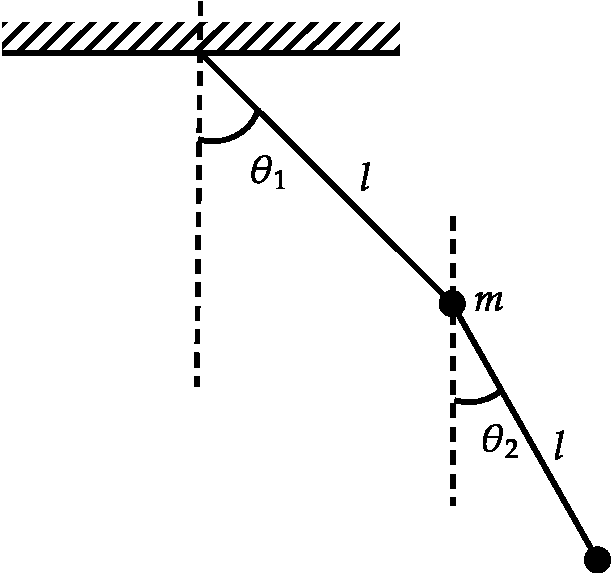
\includegraphics[height=4cm,width=4.5cm]{CM-02}
	\end{figure}
	The kinetic energy of the pendulum is :
	 \begin{tasks}(2)
		\task[\textbf{a.}]$\frac{1}{2} \mathrm{~m} \ell^{2}\left[\dot{\theta}_{1}^{2}+\dot{\theta}_{2}^{2}\right]$
		\task[\textbf{b.}]$\frac{1}{2} m \ell^{2}\left[2 \dot{\theta}_{1}^{2}+\dot{\theta}_{2}^{2}+2 \dot{\theta}_{1} \dot{\theta}_{2} \cos \left(\dot{\theta}_{1}-\dot{\theta}_{2}\right)\right]$
		\task[\textbf{c.}]$\frac{1}{2} m \ell^{2}\left[\dot{\theta}_{1}^{2}+2 \dot{\theta}_{2}^{2}+2 \dot{\theta}_{1} \dot{\theta}_{2} \cos \left(\dot{\theta}_{1}-\dot{\theta}_{2}\right)\right]$
		\task[\textbf{d.}] $\frac{1}{2} \mathrm{~m} \ell^{2}\left[2 \dot{\theta}_{1}^{2}+\dot{\theta}_{2}^{2}+2 \dot{\theta}_{1} \dot{\theta}_{2} \cos \left(\dot{\theta}_{1}+\dot{\theta}_{2}\right)\right]$
	\end{tasks}
	\begin{answer}
		\begin{align*}
	\mathrm{x}_{1}&=\ell \sin \theta_{1},  \mathrm{x}_{2}=\ell \sin \theta_{1}+\ell \sin \theta_{2} \\ \mathrm{y}_{1}&=-\ell \cos \theta_{1},  \mathrm{y}_{2}=-\ell \cos \theta_{1}-\ell \cos \theta_{2} \\ \dot{\mathrm{x}}_{1}&=\ell \cos \theta_{1} \dot{\theta}_{1},  \dot{\mathrm{y}}_{1}=\ell \sin \theta_{1} \dot{\theta}_{1}
		\end{align*}
		\begin{figure}[H]
			\centering
			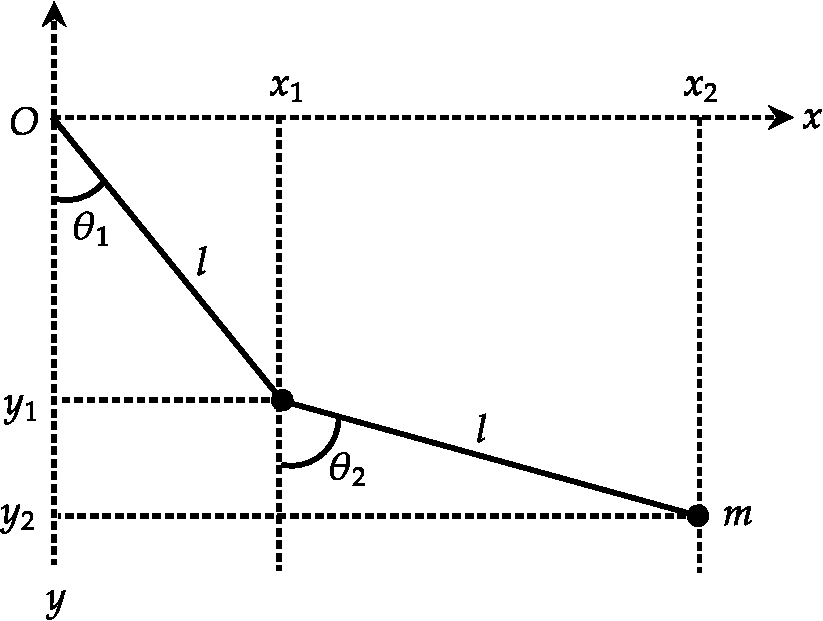
\includegraphics[height=4.5cm,width=6.5cm]{CM-03}
		\end{figure}
		\begin{align*}
		\dot{x}_{2}&=\ell \cos \theta_{1} \dot{\theta}_{1}+\ell \cos \theta_{2} \dot{\theta}_{2} ; \quad \dot{y}_{2}=\ell \sin \theta_{1} \dot{\theta}_{1}+\ell \sin \theta_{2} \dot{\theta}_{2},\\
		T&=\frac{m}{2}\left(\dot{x}_{1}^{2}+\dot{y}_{1}^{2}\right)+\frac{m}{2}\left(\dot{x}_{2}^{2}+\dot{y}_{2}^{2}\right)\\
		&=\frac{\mathrm{m}}{2} \dot{\theta}_{1}^{2} \ell^{2}+\frac{\mathrm{m}}{2}\left[\dot{\theta}_{1}^{2} \ell^{2}+\dot{\theta}_{2}^{2} \ell^{2}+2 \ell^{2} \dot{\theta}_{1} \dot{\theta}_{2} \cos \left(\theta_{1}-\theta_{2}\right)\right]\\
		&=\frac{\mathrm{m} \ell^{2}}{2}\left[2 \dot{\theta}_{1}^{2}+\dot{\theta}_{2}^{2}+2 \dot{\theta}_{1} \dot{\theta}_{2} \cos \left(\theta_{1}-\theta_{2}\right)\right]
		\end{align*}
		Correct answer is \textbf{(b)}
	\end{answer}
	\item A particle of mass ' $\mathrm{m}$ ' moves inside a bowl. If the surface of the bowl is given by the equation $\mathrm{z}=\frac{1}{2} \mathrm{a}\left(\mathrm{x}^{2}+\mathrm{y}^{2}\right)$, where $a$ is a constant, the Lagrangian of the particle is:
	 \begin{tasks}(2)
		\task[\textbf{a.}] $\frac{1}{2} m\left(\dot{r}^{2}+r^{2} \dot{\phi}^{2}-g a r^{2}\right)$
		\task[\textbf{b.}] $\frac{1}{2} m\left[\left(1+a^{2} r^{2}\right) \dot{r}^{2}+r^{2} \dot{\phi}^{2}\right]$
		\task[\textbf{c.}]$\frac{1}{2} m\left(\dot{r}^{2}+r^{2} \dot{\theta}^{2}+r^{2} \sin ^{2} \dot{\phi}^{2}-g a r^{2}\right)$
		\task[\textbf{d.}]  $\frac{1}{2} m\left[\left(1+a^{2} r^{2}\right) \dot{r}^{2}+r^{2} \dot{\phi}^{2}-g a r^{2}\right]$
	\end{tasks}
	\begin{answer}$\left. \right. $
		\begin{figure}[H]
			\centering
			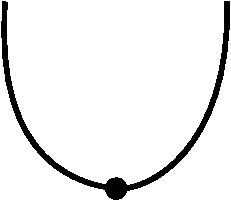
\includegraphics[height=1.5cm,width=2cm]{CM-04}
		\end{figure}
		\begin{align*}
		z&=\frac{1}{2} a\left(x^{2}+y^{2}\right)=\frac{1}{2} a r^{2} \quad \Rightarrow \dot{z}=a r \dot{r}\\
	\text{	K.E. }&=T=\frac{1}{2} m\left(\dot{x}^{2}+\dot{y}^{2}+\dot{z}^{2}\right)\\
	&=\frac{1}{2} m\left(\dot{r}^{2}+r^{2} \dot{\varphi}^{2}+\dot{z}^{2}\right)\\
	&=\frac{1}{2} m\left(\dot{r}^{2}+r^{2} \dot{\varphi}^{2}+a^{2} r^{2} \dot{r}^{2}\right) \qquad\text{ P.E.} =V=m g z=\frac{1}{2} m g a r^{2}\\
	L&=T-V=\frac{1}{2} m\left(\dot{r}^{2}+r^{2} \dot{\varphi}^{2}+a^{2} r^{2} \dot{r}^{2}-g a r^{2}\right)=\frac{1}{2} m\left[\left(1+a^{2} r^{2}\right) r^{2}+r^{2} \dot{\varphi}^{2}-g a r^{2}\right]
		\end{align*}
		Correct answer is option\textbf{(d)}
	\end{answer}
	\item A mass point glides without friction on a cycloid, which is given by $x=a(\vartheta-\sin \vartheta)$ and $y=a(1+\cos \vartheta)$ (with $0 \leq \vartheta \leq 2 \pi$ ). Determine\\
	(a) the Lagrangian, and\\
	(b) the equation of motion\\
	(c) Solve the equation of motion
	\begin{answer}
		The cycloid is represented by
		\begin{align*}
		x=a(\vartheta-\sin \vartheta), \quad y=a(1+\cos \vartheta),
		\end{align*}
		\begin{figure}[H]
			\centering
			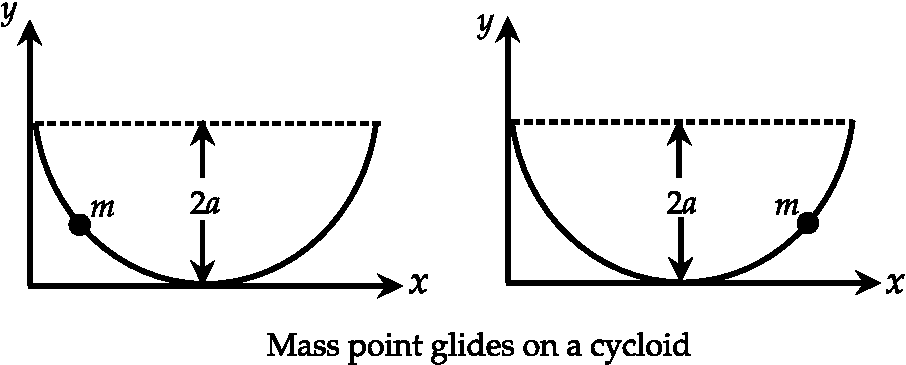
\includegraphics[height=3.2cm,width=9cm]{CM-05}
		\end{figure}
		\begin{align*}
	\text{	where }&0 \leq \vartheta \leq 2 \pi.\text{ The kinetic energy is}\\
		T=\frac{1}{2} m\left(\dot{x}^{2}+\dot{y}^{2}\right)&=\frac{1}{2} m a^{2}\left\{[(1-\cos \vartheta) \dot{\vartheta}]^{2}+[-(\sin \vartheta) \dot{\vartheta}]^{2}\right\},\\
	\text{	and the potential energy is }V&=m g y=m g a(1+\cos \vartheta).\\
		\text{The Lagrangian is given by }L&=T-V=m a^{2}(1-\cos \vartheta) \dot{\vartheta}^{2}-m g a(1+\cos \vartheta).\\
		\text{The equation of motion then reads }&\frac{d}{d t}\left(\frac{\partial L}{\partial \dot{\vartheta}}\right)-\frac{\partial L}{\partial \vartheta}=0,\\
	\text{	i.e., }\quad &\frac{d}{d t}\left[2 m a^{2}(1-\cos \vartheta) \dot{\vartheta}\right]-\left[m a^{2}(\sin \vartheta) \dot{\vartheta}^{2}+m g a \sin \vartheta\right]=0\\
	\text{ or }\quad &\frac{d}{d t}[(1-\cos \vartheta) \dot{\vartheta}]-\frac{1}{2}(\sin \vartheta) \dot{\vartheta}^{2}-\frac{8}{2 a} \sin \vartheta=0,\\
	\text{ i.e.,} \quad&(1-\cos \vartheta) \ddot{\vartheta}+\frac{1}{2}(\sin \vartheta) \dot{\vartheta}^{2}-\frac{g}{2 a} \sin \vartheta=0.\\
\text{	By setting }u&=\cos \left(\frac{\vartheta}{2}\right), \text{one has }\frac{d u}{d t}=-\frac{1}{2} \sin \left(\frac{\vartheta}{2}\right) \dot{\vartheta}\text{ and } \frac{d^{2} u}{d t^{2}}\\&=-\frac{1}{2} \sin \left(\frac{\vartheta}{2}\right) \ddot{\vartheta}-\frac{1}{4} \cos \left(\frac{\vartheta}{2}\right) \dot{\vartheta}^{2} .\\ \text{Since }&\cot \left(\frac{\vartheta}{2}\right)=\sin \frac{\vartheta}{(1-\cos \vartheta)},\text{ we can write as}\\
\ddot{\vartheta}+\frac{1}{2} \cot \left(\frac{\vartheta}{2}\right) \dot{\vartheta}^{2}-\frac{g}{2 a} \cot \left(\frac{\vartheta}{2}\right)&=0,\text{ and therefore,} \frac{d^{2} u}{d t^{2}}+\frac{g}{4 a} u=0. 
\intertext{The solution of this differential equation is}
u&=\cos \left(\frac{\vartheta}{2}\right)=C_{1} \cos \sqrt{\frac{g}{4 a}} t+C_{2} \sin \sqrt{\frac{g}{4 a}} t 
\intertext{ The motion is just like the vibration of an ordinary pendulum of length $l=4 a$. The arrangement is therefore called a "cycloid pendulum".}
		\end{align*}
	\end{answer}
	\item 	Three particles of equal mass ' $m$ ' are connected by two identical massless springs of stiffiness constant ' $k$ ' as shown in the figure.\\
	If $x_{1}, x_{2}$ and $x_{3}$ denote the displacements of the masses from their respective equilibrium positions, the potential energy of the system is:
	 \begin{tasks}(2)
		\task[\textbf{a.}]$\frac{1}{2} k\left(x_{1}^{2}+x_{2}^{2}+x_{3}^{2}\right)$
		\task[\textbf{b.}]$\frac{1}{2} k\left[x_{1}^{2}+x_{2}^{2}+x_{3}^{2}-x_{2}\left(x_{1}+x_{3}\right)\right]$
		\task[\textbf{c.}]$\frac{1}{2} k\left[x_{1}^{2}+2 x_{2}^{2}+x_{3}^{2}+2 x_{2}\left(x_{1}+x_{3}\right)\right]$
		\task[\textbf{d.}] $\frac{1}{2} k\left[x_{1}^{2}+2 x_{2}^{2}+x_{3}^{2}-2 x_{2}\left(x_{1}+x_{3}\right)\right]$
	\end{tasks}
	\begin{answer}
		\begin{align*}
		\text{Potential energy }&=\frac{1}{2} k\left(x_{2}-x_{1}\right)^{2}\hspace{2cm}
		\text{first spring}\\
	\text{	Potential energy }&=\frac{1}{2} k\left(x_{3}-x_{2}\right)^{2}\hspace{2cm}
	\text{	second spring}
	\intertext{Potential energy of the system,}
	&=\frac{1}{2} k\left(x_{2}-x_{1}\right)^{2}+\frac{1}{2} k\left(x_{3}-x_{2}\right)^{2}=\frac{1}{2} k\left[x_{1}^{2}+x_{2}^{2}-2 x_{1} x_{2}+x_{2}^{2}+x_{3}^{2}-2 x_{2} x_{3}\right]\\
	&=\frac{1}{2} k\left[x_{1}^{2}+2 x_{2}^{2}+x_{3}^{2}-2 x_{2}\left(x_{1}+x_{3}\right)\right]
		\end{align*}
		Correct answer is option \textbf{(d)}
	\end{answer}
	\item The Lagrangian of a particle of mass $m$ moving in one dimensions is given by
	$$
	\mathrm{L}=\frac{1}{2} \mathrm{~m} \dot{\mathrm{x}}^{2}-\mathrm{bx}
	$$
	where $b$ is a positive constant. The coordinate of the particle $x(t)$ at time $t$ is given by: (in the following $c_{1}$ and $c_{2}$ are constants)
	 \begin{tasks}(2)
		\task[\textbf{a.}]$-\frac{b}{2 m} t^{2}+c_{1} t+c_{2}$
		\task[\textbf{b.}]$c_{1} t+c_{2}$
		\task[\textbf{c.}]$c_{1} \cos \left(\frac{b t}{m}\right)+c_{2} \sin \left(\frac{b t}{m}\right)$
		\task[\textbf{d.}] $c_{1} \cosh \left(\frac{b t}{m}\right)+c_{2} \sin h\left(\frac{b t}{m}\right)$
	\end{tasks}
	\begin{answer}
		\begin{align*}
		L&=\frac{1}{2} m \dot{x}^{2}-b x=\mathrm{T}-\mathrm{V}\\
		\therefore \mathrm{V}&=b x
		\intertext{ This is same as uniform gravitational potential. Therefore, solution must be of the form. This is same as uniform} \mathrm{S}&=\mathrm{S}_{0}+\mathrm{ut}+\frac{1}{2} \mathrm{at}^{2}
		\end{align*}
		Correct answer is option \textbf{(a)}
	\end{answer}
	\item A particle moves in a potential $V=x^{2}+y^{2}+\frac{z^{2}}{2}$. Which component (s) of the angular momentum is $/$ are constant (s) of motion?
	 \begin{tasks}(2)
		\task[\textbf{a.}]none
		\task[\textbf{b.}]$L_{x}, L_{y}$ and $L_{z}$
		\task[\textbf{c.}]only $L_{x}$ and $L_{y}$
		\task[\textbf{d.}] only $\mathrm{L}_{z}$
	\end{tasks}
	\begin{answer}
		\begin{align*}
		\text{Given }V(x, y, z)&=x^{2}+y^{2}+\frac{z^{2}}{2}
	\intertext{	In polar co-ordinate (spherical polar)}
	V&=r^{2} \sin ^{2} \theta+\frac{r^{2} \cos ^{2} \theta}{2} \quad\left[\begin{array}{l}x=r \cos \phi \sin \theta \\ y=r \sin \phi \sin \theta \\ z=r \cos \theta\end{array}\right.
\intertext{	Therefore, Lagrangian of system is}
	\mathrm{L}&=\mathrm{T}-\mathrm{V} \\
	L&=\frac{1}{2} m\left(\dot{r}^{2}+r^{2} \dot{\theta}^{2}+r^{2} \sin ^{2} \theta \dot{\phi}^{2}\right)-r^{2} \sin ^{2} \theta-\frac{r^{2} \cos ^{2} \theta}{2}
		\end{align*}
		$\phi$ is cyclic, therefore $p_{\phi}$ is constant of motion.\\
		$p_{\phi}$ is equal to $L_{z}$. Therefore, $L_{z}$ is constant of motion.\\
		Correct answer is option \textbf{(d)}
	\end{answer}
	\item	A particle of mass $m$ is projected with an initial velocity $u$ at an angle $\alpha$ with the horizontal. Use Lagran equations to describe the motion of projectile. The resistance of air is negligible.
	\begin{answer}
			Let $x, y$ be the coordinate of the particle at any instant. The system is holonomic because its positic confined to a plane and conservative because the only external force acting on the projectile is conse tive.
		\begin{align*}
		T&=\frac{1}{2} m\left(\dot{x}^{2}+\dot{y}^{2}\right)\text{ and }V=m g y\\
		\therefore L&=T-V=\frac{1}{2} m\left(\dot{x}^{2}+\dot{y}^{2}\right)-m g v\\
		\frac{\partial L}{\partial \dot{x}}&=m \dot{x}\text{ and } \frac{\partial L}{\partial x}=0\\
		\text{By Lagrange's equation, }\frac{d}{d t}\left(\frac{\partial L}{\partial \dot{x}}\right)&=\frac{\partial L}{\partial x}\\
		\therefore \quad \frac{d}{d t}(m \dot{x})&=0 \text { or } \ddot{x} =0 \\
		\frac{\partial L}{\partial \dot{y}}&=m y \text { and } \frac{\partial L}{\partial y} =-m g\\
		\text{By Lagrange's equation }\frac{d}{d t}\left(\frac{\partial L}{\partial \dot{y}}\right)&=\frac{\partial L}{\partial y}\\
		 \therefore \quad \frac{d}{d t}(m y)&=-m g\text{ or }\ddot{y}=-g
		 \intertext{Thus, $\ddot{x}=0, \ddot{y}=-g$ are the two equations describing the motion of a projectile. Proceeding with the first equation,}
		 \frac{d}{d t}\left(\frac{d x}{d t}\right)&=0 \text { or } d\left(\frac{d x}{d t}\right)=0\\
		 \text{Integrating, }\quad \frac{d x}{d t}&=c_{1}(\text{ a constant} )\\
		\text{ At }t&=0, \quad \frac{d x}{d t}=u \cos \alpha ; \quad \therefore u \cos \alpha=c_{1}\\
		\therefore \quad \frac{d x}{d t}&=u \cos \alpha, \quad \text { or } d x=u \cos \alpha d t\\
	\text{	Integrating, }x&=(u \cos \alpha) t+x_{0}(\text{ a constant })\\
\text{	At $t=0, x=0$, }&\text{therefore, }x_{0}=0 ; x=(u \cos \alpha) t
 \intertext{Proceeding with the second equation,}
	\frac{d}{d t}\left(\frac{d y}{d t}\right)&=-g, \text { or } d\left(\frac{d y}{d t}\right)=-g d t\\
\text{	Integrating, }\frac{d y}{d t}&=-g t+c_{2}(\mathrm{a}\text{ constant })\\
	\text{At }t&=0, \frac{d y}{d t}=u \sin \alpha ; \therefore u \sin \alpha=c_{2}\\
	\therefore \quad \frac{d y}{d t}&=-g t+u \sin \alpha, o r d y=-g t d t+u \sin \alpha d t\\
\text{	Integrating, }y&=-\frac{1}{2} g t^{2}+(u \sin \alpha) t+y_{0}\\
\text{	At }t&=0, y=0\text{ and therefore, $y_{0}=0$}\\
	\therefore \quad y&=(u \sin \alpha) t-\frac{1}{2} g t^{2}
		\end{align*}
		Thus, $x=(u \cos \alpha) t, y=(u \sin \alpha) t-\frac{1}{2} g t^{2}$ are the two solved equation describing the motion of a projectile.
	\end{answer}
	\item A particle of mass $m$ is moving in a plane under the influence of a force directed towards a fixed point and varying inversely as the square of the distance from that point. Set up the Lagrangian and equations of motion of the particle.
	\begin{answer}
		The problem is best solved in polar coordinates with respect to the fixed point as origin and any line through it as the reference line. Let $(r, \theta)$ be the polar coordinates of the particle at any time. Since there are two coordinates there will be two Lagrange's equations describing the motion of the particle. Motion is holonomic because the position of the particle is confined to a plane and conservative because the force is derivable from energy or energy is derivable from the force.
		\begin{figure}[H]
			\centering
			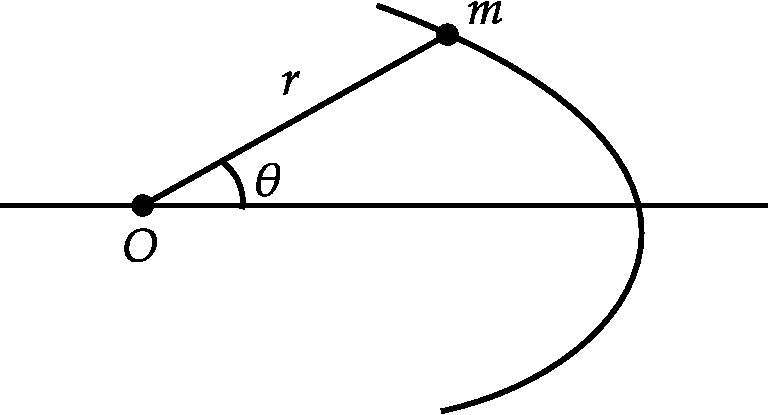
\includegraphics[height=2.5cm,width=5cm]{CM-06}
		\end{figure}
		\begin{align*}
		T&=\frac{1}{2} m \dot{r}^{2} \text{(linear kinetic energy)} +\frac{1}{2} I \dot{\theta}^{2} \text{(rotational $k$. energy)}\\
		\text{Or, }\quad T&=\frac{1}{2} m \dot{r}^{2}+\frac{1}{2}\left(m r^{2}\right) \dot{\theta}^{2} \quad\left(\because I=m r^{2}\right)
		\intertext{Since force varies inversely as the square of the distance and it is directed towards the origin, $F=-\left(k / r^{2}\right)$ where $k$ is a constant. But}
		F&=-\left(\frac{d V}{d r}\right)\\
		\therefore\quad&=\frac{k}{r^{2}}=-\frac{d V}{d r}\text{, or } d V=\frac{k d r}{r^{2}}\\
		\text{Integrating, }V&=-\frac{k}{r}+V_{0}\text{ (a constant)}\\
		\text{At }r&=\infty, V=0\text{ and therefore, }V_{0}=0 ; \therefore V=-\left(\frac{k}{r}\right)
		\end{align*}
	\end{answer}
	
	
	
	
	
\end{enumerate}